\cotefile{116}
\scanpage{2}
% archive foliation: 1
Mapping cone
\scanpage{3}
% archive foliation: 2
\diagram{\begin{tikzcd}
b\backslash A & A_0 \arrow[l]
\end{tikzcd}}
\[
\unsure{i_! = j^*}\qquad
\begin{gathered}i^*=j_*\\i_*\end{gathered}
\]
\[
p_A:A\mathbin{-}\unsure{\Delta_0|A_0}
\]
\diagram{\begin{tikzcd}[row sep=small,column sep=small]
y \arrow[r] \arrow[dd,shift left=1.5ex] & x \arrow[d]\\
b_0 \arrow[r,"p"] \arrow[d,equal] & b'\\
b_0 \arrow[ur,"p"'] &
\end{tikzcd}}
\diagram{\begin{tikzcd}
p_{A!}(F)\\
p_{A!}i_!\bigl(\unsure{G^*(F)|i^*(F)}\bigr) \arrow[u]
\end{tikzcd}}
\figure{\begin{tikzpicture}\draw (0,0)--(0,2);\end{tikzpicture}}
\diagram{\begin{tikzcd}
i_!i^*(F) \arrow[r,"\sim"] & F\\
i_*i^*F & F \arrow[l,"\sim"']
\end{tikzcd}}
\diagram{\begin{tikzcd}[column sep=large]
\widehat{A}_0 \arrow[r,shift left=2.5ex,"i_!"] \arrow[r,shift right=2.5ex,"i_*"'] & \widehat{A} \arrow[l,"i^*" description]
\end{tikzcd}}
\[
\deleted{\unsure{\varphi}}\quad
\left[\begin{array}{ll}
i^{0*}&\text{pl. fid.}\\
i^0_*&\text{localisation}\\
i^{\unsure{1|'}}_!&\text{localisation}
\end{array}\right.
\]
\[
\deleted{\unsure{\exists}}\quad\uline{E_\alpha}\quad\unsure{\ddot{u}|U}
\]
\diagram{\begin{tikzcd}
F \arrow[r] & \unsure{i^0_*i^{0*}F|i^0_*i^*F}
\end{tikzcd}}
\unsure{induit} iso sur $\Gamma$ pour $\unsure{\forall|H}\ F$

\uline{$i$ est tot} $0$-asph.
\diagram{\begin{tikzcd}
A_0 \arrow[r] & \uline{A}
\end{tikzcd}}
\scanpage{4}
% archive foliation: 3
Relation entre morphismes de topos et recollements de topos.

\margin{On remplace un morphisme \unsure{quelc.} de topos par un plongement fermé.}

1) \deleted{Soit}\inserted{Soit}
\[
(1)\qquad f:\mathcal X_0\longrightarrow\mathcal X_1\quad\deleted{\unsure{\mathcal X}}
\]
un morphisme de topos, on peut le considérer comme un topos fibré sur $\Delta_1$ (fibres $\mathcal X_0,\mathcal X_1$), et regarder le topos total associé $\mathcal X=C(f)$ \inserted{(le mapping-cone)} dont les faisceaux sont les systèmes
\[
(2)\qquad\left\{\begin{array}{ll}
(F_0,F_1,u),&F_0\in\operatorname{Ob}\mathcal F(\mathcal X_0),\ F_1\in\operatorname{Ob}\mathcal F(\mathcal X_1)\\
&u:\unsure{f_0^*|f^*}(F_1)\longrightarrow F_0\quad\text{i.e.}\\
&F_1\longrightarrow f_*(F_0)
\end{array}\right.
\]
\margin{\uline{NB} On a $\mathcal X\longrightarrow\operatorname{Top}(\Delta_1)$, ou ce qui revient au $=$, on a un $\mathcal X_0$ \unsure{comme} sous-topos ouvert (image inverse du sous-objet $\{0\}$ de l'objet final de $\widehat{\Delta}_1$).}

Alors $\mathcal X_0$ peut être regardé comme un ouvert de $\mathcal X$, $\mathcal X_1$ comme le fermé complémentaire, mais de plus l'inclusion
\[
(3)\qquad\mathcal X_1\xrightarrow{i_1}\mathcal X
\]
\uline{est strictement \deleted{asphérique}\inserted{\unsure{équiv. f.|équiv. h.}}}
i.e. pour \uline{tout} faisceau $F$ \inserted{$(F_0,F_1,u)$} sur $\mathcal X$,
\[
H^*(\mathcal X,F)\xrightarrow{\sim}H^*(\mathcal X_1,i_1^*(F)).
\]
\margin{\uline{Re NB} On a une rétraction $r$ de $\mathcal X$ sur le sous-topos fermé $\mathcal X_1$, par le foncteur
\[
r^*(F_1)=(f^*F_1\unsure{)},F_1,\deleted{\unsure{Ident.}}).
\]
\[
\mathcal X=(\mathcal X_0\times\widehat{\Delta}_1)\amalg_{(\mathcal X_0,\unsure{1|0})}\unsure{\mathcal X_1}
\]
\deleted{$\unsure{\mathcal X_0\times\widehat{\Delta}_1}$}}

\deleted{\unsure{Le}} Le ``foncteur recollement'' \inserted{(exact à g.)} (de la théorie générale
\[
\varphi:\mathcal F(\mathcal X_0)\mathbin{-}\mathcal F(\mathcal X_1)
\]
n'est autre que
\[
(4)\qquad\varphi=f_*
\]
\scanpage{5}
% archive foliation: 4
Donc: se donner un morphisme de topos \inserted{$\mathcal X_0\mathbin{-}\mathcal X_1$} revient au $=$ que de se donner un topos $\mathcal X$, \inserted{\unsure{distinguer un}} un sous-topos ouvert \inserted{$\mathcal X_0$}, et le fermé complémentaire $\mathcal X_1$, de telle façon que le foncteur recollement $\varphi$ soit, non seulement exact à g, mais commute aux $\underset{\leftarrow}{\lim}$ quelconques, \deleted{\unsure{et de}} i.e. admette un adjoint à gauche $f^*$, et que de \uline{plus} ce dernier soit exact à gauche. Alors l'inclusion $i:\mathcal X_1\longrightarrow\mathcal X$ est fort asphérique (\uline{réciproque} ?) et la suite exacte de cohomologie relative
\margin{?}
\[
(5)\quad\longrightarrow H^i_{\mathcal X_1}(\mathcal X,F)\longrightarrow H^i(\mathcal X,F)\longrightarrow H^i(\mathcal X_0,F)\longrightarrow H^{i+1}_{\mathcal X_{\unsure{1|0}}}(\mathcal X,F)\longrightarrow\cdots
\]
peut s'écrire
\[
(5')\quad\longrightarrow H^i_{\mathcal X_1}(\mathcal X,F)\longrightarrow H^i(\mathcal X_1,F_1)\longrightarrow H^i(\mathcal X_0,F_0)\longrightarrow H^{i+1}_{\mathcal X_{\unsure{1|0}}}(\mathcal X,F)\longrightarrow\cdots
\]
On \unsure{pose}
\[
H^i_{\mathcal X_1}(\mathcal X,F)\overset{\text{déf}}{=}H^i(\underbrace{\mathcal X_1\operatorname{mod}\mathcal X_0}_{\inserted{f\ \text{sous-entendu}}},F=(F_0,F_1,u))
\]
noté aussi \deleted{\unsure{en}} $H^i(\mathcal X_1\operatorname{mod}\mathcal X_0\unsure{\}},F_1)$ si $F_0=f^*(F_1)$, $u$ tautolog.
\scanpage{6}
% archive foliation: 5
Dire que $f:\mathcal X_0\longrightarrow\mathcal X_1$ est \deleted{asphérique}\inserted{équiv. faible}, \unsure{signifie} aussi que
\diagram{\begin{tikzcd}
\mathcal X_0 \arrow[r] \arrow[r,shift right=2ex] \arrow[dr] & \mathcal X\\
& \mathcal X_1 \arrow[u,"\unsure{\sim}"']
\end{tikzcd}}
(imm. ouverte) l'est. (\uline{NB} Les faisceaux loc. constants sur $\mathcal X$ sont ceux de la forme $(F_1,f^*(F_1),u\ \text{tautol.})$, avec $F_1$ loc. ct. sur $\unsure{\mathcal X_0|\mathcal X_1}$.)

2) Partons inversement d'un topos $\mathcal X$, et d'un sous-topos ouvert
\[
(6)'\qquad\mathcal X_0\subset\mathcal X,
\]
$\unsure{\Longleftrightarrow|\Longleftarrow}$ sous-objet de l'objet final $e_{\mathcal X}$ de $\mathcal F(\mathcal X)$, d'où topos résiduel $\mathcal X_1$. On peut considérer aussi que la donnée de $\mathcal X_0$ correspond à celle d'un morphisme
\[
\pi:\mathcal X\longrightarrow\operatorname{Top}(\Delta_1)
\]
$\mathcal X_0$ étant l'image inverse du sous-topos ouvert ``universel'' $\{0\}$ dans $\operatorname{Top}(\Delta_1)$, et $\mathcal X_1$ de \deleted{\unsure{de}} l'image inverse du sous topos fermé $\{1\}$.
\scanpage{7}
% archive foliation: 6
D'autre part, la donnée de $(\mathcal X,\mathcal X_0)$ équivaut à celle de
\[
(\mathcal X_0,\mathcal X_1,\varphi)\qquad
\overset{\substack{\inserted{[f_*]}\\\Vert}}{\varphi}:\mathcal F(\mathcal X_0)\longrightarrow\mathcal F(\mathcal X_1)
\]
foncteur exact à g. \inserted{``accessible''}

On \unsure{s'intéresse|s'intéressera} à des conditions \inserted{sur $(\mathcal X_0,\mathcal X_1,\varphi)$} qui assurent que les \inserted{deux} inclusions
\diagram{\begin{tikzcd}
\mathcal X_0 \arrow[r] & \mathcal X & \mathcal X_1 \arrow[l]
\end{tikzcd}}
sont des équivalences faibles. Les cas qui nous intéressent le plus, sont les cas où $\varphi\inserted{=f_*}$ commute en fait aux $\underset{\leftarrow}{\lim}$ quelconques \inserted{i.e. a un adjoint à droite $f^*$}, --- comme p.ex. celui du § précédent, où on supposait \uline{de plus} que $f^*$ est exact à gauche (mais on \uline{n'a} \uline{pas} envie de le supposer ici). Un cas particulièrement important pour nous est celui où $\mathcal X$ est de la forme $\deleted{\unsure{\widehat X}}\inserted{\operatorname{Top}(X)}$, un $X$ dans $(\operatorname{Cat})$, il revient au $=$ de dire que
\scanpage{8}
% archive foliation: 7
$\mathcal X_0,\mathcal X_1$ sont de la forme $\deleted{\unsure{\widehat X_0,\widehat X_1}}\inserted{\operatorname{Top}(X_0),\operatorname{Top}(X_1)}$, et que $\varphi$ commute aux $\underset{\leftarrow}{\lim}$ quelconques i.e. a un adjoint à g. $f^*$, qui est donc défini par un foncteur
\[
X_1\longrightarrow\widehat X_0
\]
(se prolongeant par ``continuité'' via $\underset{\longrightarrow}{\lim}$ en
\[
\widehat X_1\xrightarrow{f^*}\widehat X_0
\]
), correspondant à un bifoncteur
\[
(x_0,x_1)\longmapsto h(x_1,x_0),\qquad X_0^{\mathrm{op}}\times X_1\longrightarrow(\operatorname{Ens}).
\]
\scanpage{10}
% archive foliation: 9
\diagram{\begin{tikzcd}
A \arrow[d] & A' \arrow[l] \arrow[d]\\
B & B' \arrow[l]
\end{tikzcd}}
$A$ fibrant
\diagram{\begin{tikzcd}
A_{/b} \arrow[r,phantom,"\unsure{\rightleftarrows|\hookleftarrow}" description] & A_b
\end{tikzcd}}
\[
\left|\begin{gathered}
\underset{\substack{\leftarrow\\A_{/b}}}{\lim}(F\mid A_{/b})\xrightarrow{\uline{\mathrm{iso}}}\underset{\substack{\leftarrow\\A_b}}{\lim}F\mid A_b\\
\text{Pour }\unsure{\forall|\mathrm{tt}}\ F\text{ sur }A\text{ (ou sur }A_{/b}\text{)}
\end{gathered}\right.
\]
\diagram{\begin{tikzcd}
\unsure{i_b|j_b}\arrow[d,no head]\\
{}
\end{tikzcd}}
\margin{$\displaystyle\int$ dans $\operatorname{Hot}$}
\scanpage{11}
% archive foliation: 10
\begin{center}
U N I V E R S I T E\\
DES SCIENCES ET TECHNIQUES\\
DU LANGUEDOC\\
\texttt{-{}-{}-{}-{}-{}-{}-{}-{}-{}-{}-{}-{}}

Service de la Scolarité\\
MA / GJ\\
Diffusion : Liste A\\
N° : 3547
\end{center}

MONTPELLIER, le 19 JUIN 1981

AVIS DE SOUTENANCE D'UN \unsure{DIPLOME|DIPLÔME} D'ETUDES SUPERIEURES D'UNIVERSITE

\texttt{-{}-{}-{}-{}-{}-{}-{}-{}-{}-{}-{}-{}-{}-{}-{}-{}-{}-{}-{}-{}-{}-{}-{}-{}-{}-{}-{}-{}-{}-{}-{}-{}-{}-{}-{}-{}-{}-{}-{}-{}-{}-{}-{}-{}-{}-{}-{}-{}-{}-{}-{}-{}-{}-{}-{}-{}-{}-{}-{}-{}-{}-{}-{}-{}-{}}

Le 30 JUIN 1981 à 16 heures 30 mn

A L'ECOLE NATIONALE SUPERIEURE DE CHIMIE\\
(Amphi Gerhard)

Monsieur EL MANSOURI Abdeslam

soutiendra un Diplôme d'Etudes Supérieures d'Université portant sur le sujet suivant :

``Contribution à l'étude des systèmes binaires $\mathrm{PbF}_2$ - $\mathrm{SnF}_4$ et $\mathrm{PbF}_2$ - $\mathrm{GeF}_4$''.

\uline{Membres du jury} :
\begin{tabular}{ll}
MM.&COT L.\\
&RIBES M.\\
&LIVAGE L.\\
&GRANIER W.\\
&VIMINOT S.
\end{tabular}

P. le Secrétaire Général,\\
l'Attachée d'Administration Universitaire,

\unsure{Gentil}
\figure{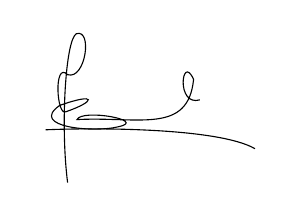
\begin{tikzpicture}[x=1cm,y=1cm]
\draw (0.2,-0.55) .. controls (0.11,0.15) and (0.17,1.25) .. (0.31,1.34)
.. controls (0.52,1.41) and (0.43,0.75) .. (0.20,0.82)
.. controls (0.02,1.00) and (0.06,0.28) .. (0.18,0.35)
.. controls (0.56,0.48) and (0.58,0.60) .. (0.10,0.43)
.. controls (-0.30,0.15) and (0.55,0.08) .. (0.85,0.16)
.. controls (1.22,0.24) and (0.38,0.39) .. (0.32,0.25)
.. controls (1.11,0.29) and (1.73,0.06) .. (1.80,0.76)
.. controls (1.65,1.10) and (1.57,0.41) .. (1.88,0.50);
\draw (-0.08,0.12) .. controls (0.62,0.15) and (2.13,0.14) .. (2.58,-0.12);
\end{tikzpicture}}
A. GENTIL
\cotefile{117}
\scanpage{2}
\uline{Structure des dérivateurs}
\margin{\uline{déc. 83}}
\deleted{Hom}

Dans $\mathcal H(I)$,
\[
\begin{aligned}
(1)\quad&\operatorname{Hom}(x,y)\in\operatorname{Ens}\\
(2)\quad&\unsure{\operatorname{Homht}|\operatorname{Homhot}}(x,y)\in(\operatorname{Hot})\\
(3)\quad&\boxed{\uline{\unsure{\operatorname{Homht}|\operatorname{Homhot}}}(x,y)\in\operatorname{Hot}_{\deleted{\unsure{\widehat I}}}(I)}
\end{aligned}
\]
\[
\operatorname{Hom}(x,y)\simeq\pi_0\bigl(\unsure{\operatorname{Homht}|\operatorname{Homhot}}(x,y)\bigr)
\]
\[
\unsure{\operatorname{Homht}|\operatorname{Homhot}}(x,y)\simeq\int_I\uline{\unsure{\operatorname{Homht}|\operatorname{Homhot}}}(x,y).
\]
\margin{$\begin{gathered}-\\-\end{gathered}$}

Soit $f:I\longrightarrow J$, on a pour $X$ dans $\mathcal H(I)$, $Y$ dans $\mathcal H(J)$,
\[
\left\{\begin{aligned}
(1')\quad&\operatorname{Hom}(f_!(X),Y)=\operatorname{Hom}(X,f^*Y)\\
(2')\quad&\unsure{\operatorname{Homht}|\operatorname{Homhot}}(f_!(X),Y)\simeq\unsure{\operatorname{Homht}|\operatorname{Homhot}}(X,f^*(Y))\\
(3')\quad&\boxed{\uline{\unsure{\operatorname{Homht}|\operatorname{Homhot}}}(f_!X,Y)\simeq f_*\uline{\unsure{\operatorname{Homht}|\operatorname{Homhot}}}(X,f^*(Y))}
\end{aligned}\right.
\]
\margin{adjonction}
\margin{\unsure{est|et} \unsure{formule complète}, donne \unsure{précédente|précédent} en passant aux $\unsure{\pi_0}$.}
\margin{donne $(2')$ en intégrant $\displaystyle\int_J$}
\margin{duales}

De $=$
\[
\left\{\begin{aligned}
(1'')\quad&\operatorname{Hom}(f^*(Y),X)\simeq\operatorname{Hom}(Y,f_*(X))\\
(2'')\quad&\unsure{\operatorname{Homht}|\operatorname{Homhot}}(f^*(Y),X)\simeq\unsure{\operatorname{Homht}|\operatorname{Homhot}}(Y,f_*(X))\\
(3'')\quad&\boxed{\uline{\unsure{\operatorname{Homht}|\operatorname{Homhot}}}(\deleted{\unsure{f^*}}Y,\inserted{f_*}X)\simeq f_*\uline{\unsure{\operatorname{Homht}|\operatorname{Homhot}}}(\inserted{\unsure{f^*}}Y,X)}
\end{aligned}\right.
\]

% Two unlabelled curved annotation strokes across the signs in (1'') and (2'').
\figure{\begin{tikzpicture}[x=1cm,y=1cm]
\draw (0,0) .. controls (.45,-.30) and (.95,-.29) .. (1.08,.02)
.. controls (1.17,.31) and (1.08,.89) .. (1.42,1.05)
.. controls (1.66,1.14) and (1.89,1.09) .. (1.91,.89);
\draw (.92,-.95) .. controls (1.26,-1.13) and (1.35,-1.09) .. (1.42,-.58)
.. controls (1.46,-.06) and (1.54,.05) .. (1.87,.04)
.. controls (2.14,.05) and (2.38,.15) .. (2.39,-.10);
\end{tikzpicture}}
\scanpage{3}
% archive foliation: 2
\[
\pi_0(x,y)=\operatorname{Hom}_H(x,y)
\]
\diagram{\begin{tikzcd}x\arrow[r,"f"]&y\end{tikzcd}}
\[
\pi_1(x,y;f)=\deleted{\unsure{\pi_0\operatorname{Aut}f}}
\]
\[
H(\Delta_1)
\]
\diagram{\begin{tikzcd}{}\arrow[d]\\{}\end{tikzcd}}
\diagram{\begin{tikzcd}{}\arrow[r]&{}\arrow[r]&{}\arrow[r]&{}\end{tikzcd}}
\[
H(\Delta_1)\longrightarrow H(\Delta_0)\times H(\Delta_0)
\]
\diagram{\begin{tikzcd}\varphi\arrow[r]&{}\end{tikzcd}}
\diagram{\begin{tikzcd}x\arrow[r,bend left=45]&y\end{tikzcd}}
\[
M\quad W
\]
\diagram{\begin{tikzcd}{}\arrow[r]&{}\end{tikzcd}}
\[
\operatorname{Hot}
\]
\[
J\subset I\qquad X_J\qquad\mathcal H(J)
\]
\[
\deleted{\unsure{\operatorname{Ch}_W}(x,y)=}
\]
\[
\mathcal H(I,J)
\]
\diagram{\begin{tikzcd}[column sep=large]
\bullet\arrow[r,bend left=35,""{name=U,below}]\arrow[r,bend right=25,""{name=D,above}]&\bullet
\arrow[from=U,to=D,shift left=3pt]\arrow[from=U,to=D,shift right=3pt]
\end{tikzcd}}
\[
\unsure{H}\quad\mathcal H(I)\longrightarrow\mathcal H(J)
\]
\diagram{\begin{tikzcd}x\arrow[r]&y\end{tikzcd}}
\diagram{\begin{tikzcd}x\arrow[r,leftrightarrow]&y\end{tikzcd}}
\[
X_i\mathbin{-}X_j
\]
\diagram{\begin{tikzcd}x\arrow[r]&y\end{tikzcd}}
\[
Y_i\longrightarrow Y_j
\]
\diagram{\begin{tikzcd}[column sep=large]
x\arrow[r,bend left=35,"f",""{name=U,below}]\arrow[r,bend right=35,"g"',""{name=D,above}]&y
\arrow[from=U,to=D,"\unsure{\alpha}" description]
\end{tikzcd}}
\[
\deleted{\unsure{\xi}}\quad\Pi_1(X,Y;f,g)
\]
\diagram{\begin{tikzcd}[column sep=large]
x\arrow[r,bend left=35,""{name=U,below}]\arrow[r,bend right=35,""{name=D,above}]&y
\arrow[from=U,to=D]
\end{tikzcd}}
\diagram{\begin{tikzcd}x\arrow[r,bend left=35]\arrow[r,bend right=35]&y\end{tikzcd}}
\diagram{\begin{tikzcd}[row sep=small,column sep=small]
&{}&{}\arrow[l]\arrow[r]&{}&\\
x\arrow[ur]&&&&y\arrow[ul]\arrow[dl,bend left=15]\\
&{}\arrow[ul]&{}\arrow[l]\arrow[r]&{}\arrow[ur]&
\end{tikzcd}}
\diagram{\begin{tikzcd}\bullet&\bullet\end{tikzcd}}
\diagram{\begin{tikzcd}[column sep=huge]
x\arrow[r,bend left=40,""{name=U,below}]
\arrow[r,leftrightarrow,bend right=40,""{name=D,above}]&y
\arrow[from=U,to=D,bend right=20,shift left=5pt,""{name=L,right}]
\arrow[from=U,to=D,bend left=20,shift right=5pt,""{name=R,left}]
\arrow[from=L,to=R]
\end{tikzcd}}
\[
x\qquad y
\]
\deleted{Hom}
\[
\operatorname{Cl}(M,W)
\]
\unsure{simplexes purs|simples purs}
\diagram{\begin{tikzcd}[column sep=large]
\bullet\arrow[r,bend left=45]\arrow[r,bend right=15]\arrow[r,bend right=65]&\bullet
\end{tikzcd}}
\margin{\unsure{M}\ \illegible{2}\ \unsure{(Cat)}}
\scanpage{4}
% Archive foliation: 3, lower right. No secure authorial page number.
\margin{$\{$}
a) Modèles -- leur importance, leur indétermination

\margin{$\left\{\vphantom{\begin{matrix}b\\c\end{matrix}}\right.$}
b) Suites exactes longues (\unsure{coh.} de deux types) associées
à une flèche -- \unsure{liés|liées} à la construction des cylindres
\deleted{\unsure{de|et}} et cocylindres d'un objet-modèle, et du cylindre
et cocylindre d'une application entre modèles

\textcircled{c)} Notion de résolution d'un modèle (gauche ou droite)
formalisme des foncteurs dérivés (quand il y a
\inserted{deux th. homotopiques en présence})

\margin{$\left\{\vphantom{\begin{matrix}d\\e\end{matrix}}\right.$}
d) Notions homotopiques sur modèles (structure
homotopique: appl. homotopes, homotopismes\ldots)
``Résolutions définies à homotopie près''.
\margin{mais ce sont des notions \uline{indispensables}
pour la construction des cat. dérivées}

e) Homotopies entre applications, homotopies entre
homotopies etc. On a sans doute
\deleted{\unsure{une application}} pour deux modèles
$X,Y$ un objet $\uline{\operatorname{Hom}}(X,Y)$ dans $\mathrm{Hot}$
\unsure{voire} $=$ un complexe \inserted{\unsure{h. simplicial|h. simpl.}} de type convenable
explicite lui donnant naissance
-- et dans $\mathcal H$ un $\operatorname{Hom}$ externe à valeurs dans
$\mathrm{Hot}\ldots$, ou dans une théorie plus riche
(dans laquelle il y a des $\operatorname{Hom}$ \unsure{h simpliciaux}).

\deleted{f) Cf plus bas}
\margin{\figure{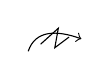
\begin{tikzpicture}[scale=.45]
\draw[->] (0,0) .. controls (.2,.6) and (.8,.6) .. (1.5,.35);
\draw (0.35,.2)--(.85,.65)--(.75,.1)--(1.15,.4);
\end{tikzpicture}}}
\margin{$\left\{\vphantom{\begin{matrix}f\\g\end{matrix}}\right.$}
\deleted{\unsure{g)}}\inserted{\unsure{f)}} Opérations de troncature, soit grossières
sur modèles, soit délicates sur $\mathcal H$.

\deleted{\unsure{h)}}\inserted{\unsure{g)}} Invariants $\pi_i$ ou $H_i$, à valeurs dans
une catégorie (souvent abélienne) associée
à la théorie.
\margin{f) et g) sont des opérations particulièrement \unsure{peu comprises}.}
\margin{\figure{\begin{tikzpicture}[scale=.4]\draw[line width=.6pt] (0,.4)--(.4,.4)--(.4,0);\end{tikzpicture}}}
\scanpage{5}
% Archive foliation: 4, lower left.
\unsure{i)|h)} Possibilité de définir \unsure{des|un} invariants
$K(\mathcal H)$ via ``triangles exacts'', voire $K_n$
supérieurs d'une théorie homotopique.
\margin{(Cas additif seulement ?!?)}
\margin{\figure{\begin{tikzpicture}[scale=.5]\draw[<->] (0,3)--(1.2,0);\end{tikzpicture}}}

\deleted{\unsure{j)}}\inserted{h)} Souvent il y a \inserted{des} $\uline{\operatorname{Hom}}$ internes
dans $\mathcal H$, avec \deleted{\unsure{des}}\inserted{une} formule du type
\[
\operatorname{Hom}(\unsure{f|\xi},\unsure{g|\eta})
=\Gamma\,\uline{\operatorname{Hom}}(\unsure{f|\xi},\unsure{g|\eta})\unsure{)|\}}
\]
\margin{Structure multiplicative et structure $\operatorname{Hom}$}
\[
\Gamma\text{ ou }\pi_0:\mathcal H\longrightarrow\mathrm{Ens}
\]
un foncteur \unsure{important|imposé} (souvent
$\operatorname{Hom}(1,-)$, où $1$ un objet unité\ldots)
\margin{(24.11.83) Relations entre ces $\uline{\operatorname{Hom}}$ internes et les
$\uline{\operatorname{Homhot}}(x,y)\in\operatorname{Ob}\mathrm{Hot}$
dans e) ??}

Souvent aussi, Structure multiplicative
(soit produit cartésien, soit un produit $\otimes$)
avec une formule
\[
\operatorname{Hom}(x\otimes y,z)\simeq
\operatorname{Hom}(x,\uline{\operatorname{Hom}}(y,z))
\]
\figure{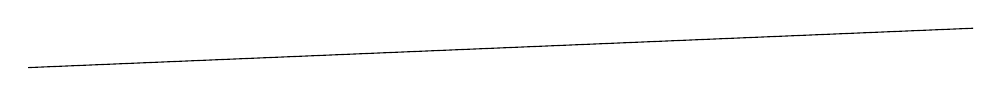
\begin{tikzpicture}\draw (0,0)--(12,.5);\end{tikzpicture}}
Sauf peut-être les Structures
f) et g), il semble que tout puisse
se décrire en termes de $(M,W\subset\operatorname{Fl}(M))$.
\uline{Dégager les bons axiomes}
\scanpage{6}
\mspage{1}
% Archive foliation: 5, lower left.
Théorie (de variance) homotopique $\mathcal H$.
\margin{\textcircled{1} \uline{Variance}}
Elle associe à toute \inserted{petite}\deleted{\unsure{petite}} catégorie
$A\deleted{\in\operatorname{Ob}\mathrm{Cat}}$,
\margin{\deleted{(pas néc. petite)}}
une catégorie
(pas néc. petite\deleted{$\unsure{\mathcal H}$}\deleted{, $=$ si $A$ l'est})
\[
(1)\qquad \boxed{A\longmapsto\mathcal H(A)}
\]
\margin{\figure{\begin{tikzpicture}[scale=.3]\draw (0,.2) .. controls (.5,.5) and (.8,.4) .. (.9,0);\end{tikzpicture}}}
\deleted{et de plus pour $f$}
qui est $2$-contravariante en $A$ (de façon \uline{stricte})
\[
(2)\qquad
\underset{\substack{\text{foncteur}\\\text{entre $\mathcal U$-catégories}}}{f:A\longrightarrow B}
\quad\text{implique}\quad
\mathcal H(B)\xrightarrow{f_{\mathcal H}^{*}}\mathcal H(A)
\]
(\unsure{à préciser|bien préciser}). On pose
\[
(3)\qquad \mathcal H(\Delta_0)=\mathrm{Hot}_{\mathcal H}
\]
d'où on a pour \deleted{\unsure{tout}} $A$ un foncteur
\[
(4)\qquad
\begin{aligned}
\mathcal H(A)&\xrightarrow{\alpha_A}
\uline{\operatorname{Hom}}(A,\deleted{\unsure{\mathrm{Cat}}}\mathrm{Hot}_{\mathcal H})\\
\unsure{\mathcal X|X}&\longmapsto(a\longmapsto(i_a)_{\mathcal H}^{*}(\unsure{\mathcal X|X}))
\end{aligned}
\]
où $i_a:\Delta_0\longrightarrow A$ foncteur de valeur $a$

(\uline{NB} Pour $\forall\ B$, on a
\[
\uline{\operatorname{Hom}}(B,A)\longrightarrow
\uline{\operatorname{Hom}}(\mathcal H(A),\mathcal H(B))
\]
d'où
\[
\mathcal H(A)\longrightarrow
\uline{\operatorname{Hom}}(\uline{\operatorname{Hom}}(B,A),\mathcal H(B))
\]
si $B=\Delta_0$, on trouve (4).)

Pour $f:A\longrightarrow B$
morphisme de catégories, on a une
\scanpage{7}
% Archive foliation: 6, lower left in original scan. Writing rotated 90 degrees.
% Reused administrative account sheet; ruled blank spaces retained schematically.
\diagram{\begin{tabular}{rl|c@{\qquad}rl|c}
M. \unsure{Lefranc}&\shortstack{Fixe\\Points}&$\}$&M. Hakim&\shortstack{Fixe\\Points}&$\}$\\\hline
$1\,267,00$&M. Nguiffo Boyom&&$1\,700,00$&M. Hakim&\\\cline{4-4}
$1\,267,00$&M. Laborde&&$1\,700,00$&Total&\\
$652,50$&M. \unsure{Nguiffo} Boyom&&&&\\
$443,00$&M. Malgoire&&&&\\
$1\,141,00$&M. Dufour&&&&\\
$1\,141,00$&M. Nguiffo Boyom&&&&\\\cline{1-1}
$5\,911,50$&Total&&&&\\[6cm]\hline
\end{tabular}}
\scanpage{8}
\mspage{2}
% Archive foliation: 7, lower left. Long oblique strokes cancel the lower draft, beginning with Pour.
(5)
\diagram{\begin{tikzcd}[column sep=large,row sep=large]
\mathcal H(B)\arrow[r,"\mathcal H(f)"]\arrow[d,"\alpha_B"']&\mathcal H(A)\arrow[d,"\alpha_A"]\\
\uline{\operatorname{Hom}}(B,\mathrm{Hot}_{\mathcal H})\arrow[r,"f_{(\mathrm{Hot}_{\mathcal H})}^{*}"']&\uline{\operatorname{Hom}}(A,\mathrm{Hot}_{\mathcal H})
\end{tikzcd}}
\textcircled{Hot 1} si $A=\coprod_{i\in I}A_i$, alors
$\mathcal H(A)\xrightarrow{\sim}\prod_{i\in I}\mathcal H(A_i)$ \uline{iso}

\margin{\textcircled{2} $\int$}
(\unsure{Intégration}).

\deleted{
Pour \deleted{toute} \inserted{flèche $f:A\longrightarrow B$}
\deleted{$A$ petite, i.e. $A\in\operatorname{Ob}\mathrm{Cat}$, on donne}
\[
(6)\qquad \boxed{\mathcal H(A)\xrightarrow{\uline L_A}\mathcal H(\widehat A)}
\]
rendant commutatif
\margin{\uline{Hot \unsure{2}}}
(7)
\diagram{\begin{tikzcd}[column sep=large]
\mathcal H(A)\arrow[r,"\uline L_A"]\arrow[rr,bend right=25,"\operatorname{id}_{\mathcal H(A)}"']&
\mathcal H(\widehat A)\arrow[r,"\unsure{(\epsilon_A^*)_{\mathcal H}^{*}|(\epsilon_A)_{\mathcal H}^{*}}"]&\mathcal H(A)
\end{tikzcd}}
\margin{\deleted{$\unsure{\alpha_B|f_B}$}}
où
\[
\epsilon_A:A\hookrightarrow\widehat A
\]
est l'inclusion canonique.

\uline{Hot 3} $\forall\ f:A\longrightarrow B$ dans $\mathrm{Cat}$,
$\exists\ f_!:\mathcal H(A)\longrightarrow\mathcal H(B)$
tel qu'on ait commutativité à isom près de,

(8)
\diagram{\begin{tikzcd}[column sep=large,row sep=large]
\mathcal H(A)\arrow[r,"\uline L_A"]\arrow[d,"f_!"']&
\mathcal H(\widehat A)\arrow[d,"\unsure{(f_{\widehat{\ }}^{*})_{\mathcal H}^{*}|(\widehat f^{*})_{\mathcal H}^{*}}\overset{\mathrm{def}}{=}\widehat f_!"]\\
\mathcal H(B)\arrow[r,"\uline L_B"']&\mathcal H(\widehat B)
\end{tikzcd}}
}
\scanpage{9}
% Archive foliation: 8, lower left. Writing rotated 90 degrees.
% Reused administrative account sheet; blank ruled spaces retained schematically.
\diagram{\begin{tabular}{rl|c@{\qquad}rl|c}
M. Grothendieck&\shortstack{Fixe\\Points}&$\}$&M. Charles&\shortstack{Fixe\\Points}&$\}$\\\hline
---&&&$858,00$&M. Charles&\\\cline{4-4}
&&&$858,00$&Total&\\[7cm]\hline
\end{tabular}}
\scanpage{10}
\mspage{3}
% Archive foliation: 9, upper left.
On suppose

(Hot 2) $\forall\ f:A\longrightarrow B$ dans $\mathrm{Cat}$, le foncteur
\deleted{$f^*:\unsure{\mathcal H(A)}$}
\[
f_{\mathcal H}^{*}:\mathcal H(B)\longrightarrow\mathcal H(A)
\]
a un \uline{adjoint à gauche}
\[
f_!^{\mathcal H}:\mathcal H(B)\longrightarrow\mathcal H(A)
\]
de sorte que $\mathcal H(A)$ devient aussi \uline{covariant} en
$A$.
Il faut faire Attention, s'il ne faudrait pas
se borner ici aux $f$ \uline{cofibrants}.
\margin{\uline{voir}}

Si $B=\Delta_0$, on trouve
\[
\mathcal H(A)\longrightarrow\mathrm{Hot}_{\mathcal H}
\]
\margin{où $\pi_A:A\longrightarrow\Delta_0$ la projection}
\margin{$(\pi_A)_!$}
noté $\int_A$, et appelé foncteur intégration
jouant le rôle \unsure{de un|d'un} $\underset{A}{\underset{\longrightarrow}{\lim}}$.

On en a donc, par transitivité
\[
\int_A\mathcal X=\int_B f_!(\mathcal X
\]
\[
f:A\longrightarrow B.
\]
\margin{NB L'existence des $f_!$ implique l'existence
des sommes dans les $\mathcal H(A)$, $\unsure{\leftarrow|<}$,
\deleted{$\unsure{f}$} \unsure{Bien sûr} les $f_!$ y \unsure{commutent}.}
\margin{\figure{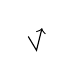
\begin{tikzpicture}[scale=.35]\draw[->] (0,.5)--(.3,0)--(.5,.8);\end{tikzpicture}}}

\textcircled{3} Opérations $\prod_A$ de cointégration,
\margin{\textcircled{Hot 3}}
par des $f_*^{\mathcal H}$ adjoints à droite des $f_{\mathcal H}^{*}$.
\scanpage{11}
% Archive foliation: 10, lower left. Writing rotated 90 degrees.
% Reused administrative account sheet; blank ruled spaces retained schematically.
\diagram{\begin{tabular}{rl|c@{\qquad}rl|c}
M. Micali&\shortstack{Fixe\\Points}&$\}$&M. Maisonneuve&\shortstack{Fixe\\Points}&$\}$\\\hline
$966,00$&M. Micali&&$400,00$&M. Maisonneuve&\\
$789,50$&M. Boé&&$1\,073,20$&M. Maisonneuve&\\
$373,25$&M. \unsure{Meffroy|Meffoy}&&$500,00$&M. \unsure{Pinchaud|Pinchard}&\\
$326,23$&M. \unsure{Meffroy|Meffoy}&&$792,00$&M. \unsure{Pinchaud|Pinchard}&\\
$617,00$&M. Revoy&&$\unsure{330,70|830,70}$&M. Maisonneuve&\\\cline{4-4}
$1\,175,00$&M. Micali&&$3\,095,90$&Total&\\
$409,57$&M. Micali&&&&\\
$592,50$&M. Micali&&&&\\
$634,50$&M. Micali&&&&\\\cline{1-1}
$5\,883,55$&Total&&&&\\[4cm]\hline
\end{tabular}}
\scanpage{12}
\mspage{4}
% Archive foliation: 11, lower left.
On déduit des foncteurs
\[
\underset{\substack{\Vert\\(\pi_A)_*}}{\prod_A}:\mathcal H(A)\longrightarrow\mathrm{Hot}_{\mathcal H}
\]
et
\[
\prod_A\mathcal X=\prod_B f_*(\mathcal X).
\]
\margin{L'existence des $f_*^{\mathcal H}$ implique celle des
produits dans les $\mathcal H(A)$.
Les $f_*$ y commutent.}

\uline{Dualité} Posons $\mathcal H^{\circ}(A)=\mathcal H(A)^{\circ}$, on trouve
des
\[
\unsure{f_{\mathcal H^{\circ}}^{\circ *}|f_{\mathcal H^{\circ}}^{*}}
=(f_{\mathcal H}^{*})^{\circ}:\mathcal H^{\circ}(B)\longrightarrow\mathcal H^{\circ}(A),
\]
et
\[
\left\{\begin{aligned}
f_!^{\mathcal H^{\circ}}&=(f_*^{\mathcal H})^{\circ}\\
f_*^{\unsure{\mathcal H|\mathcal H^{\circ}}}&=(f_!^{\mathcal H})^{\circ}
\end{aligned}\right.
\]
Les opérations $\int$ et $\prod$ s'échangent.

\uline{Cas additif} Les $\mathcal H(A)$ \deleted{\unsure{ab.}} cat. additives
\unsure{(resp.|Comp.} $k$-linéaires, $k$ anneau fixé), $f_{\mathcal H}^{*}$
additifs, alors les $f_!^{\mathcal H},f_*^{\mathcal H}$ additifs.
\scanpage{13}
% Archive foliation: 12, lower left. Writing rotated 90 degrees opposite to scans 007, 009, 011.
% Reused administrative account sheet; blank ruled spaces retained schematically.
\diagram{\begin{tabular}{rl|c@{\qquad}rl|c}
M. Roby&\shortstack{Fixe\\Points}&$\}$&M. Nouazé&\shortstack{Fixe\\Points}&$\}$\\\hline
$1\,096,00$&M. \unsure{Thérond|Théond}&&---&&\\
$1\,198,00$&M. \unsure{Thérond|Théond}&&&&\\\cline{1-1}
$2\,294,00$&Total&&&&\\[7cm]\hline
\end{tabular}}
\scanpage{14}
\mspage{5}
% Archive foliation: 13, lower right.
\uline{Ex 1} $M$ catégorie, avec $\underset{\longrightarrow}{\lim}$ et $\underset{\longleftarrow}{\lim}$
quelconques. On pose
\[
\mathcal H(A)=\uline{\operatorname{Hom}}(A,M)
\]
Alors on sait que les foncteurs
\[
f_M^{*}:\underset{\substack{\Vert\\\mathcal H(B)}}{\uline{\operatorname{Hom}}(B,M)}
\longrightarrow
\underset{\substack{\Vert\\\mathcal H(A)}}{\uline{\operatorname{Hom}}(A,M)}
\]
associés aux $f:A\longrightarrow B$ dans $\mathrm{Cat}$, admettent
des adjoints à g. $f_!^M$ et à dr. $f_*^M$,
Ici $\mathrm{Hot}_{\mathcal H}=M$ -- ce cas est
considéré trivial.
\margin{Ici $\left\{\begin{aligned}
\int_A&=\underset{A}{\underset{\longrightarrow}{\lim}}\\
\prod_A&=\underset{A}{\underset{\longleftarrow}{\lim}}
\end{aligned}\right.$}

\uline{Ex 2} Soit $(M,W)$, avec $W\subset\operatorname{Fl}(M)$.
On définit
\[
\unsure{\mathcal W_A|W_A}\subset\operatorname{Fl}\uline{\operatorname{Hom}}(A,M)
\]
\deleted{\unsure{par}} équiv. fibre par fibre, et on
\inserted{pose}
\[
\mathcal H(A)=W_A^{-1}\uline{\operatorname{Hom}}(A,M)
\]
La formation des $f_{\mathcal H}^{*}$ est évidente.
\margin{Attention, \unsure{il n'est pas clair} ici que
$\mathcal H(\coprod A_i)\xrightarrow{\sim}\prod_I\mathcal H(A_i)$,
\unsure{sauf} pour $I$ fini.}
\scanpage{15}
% Archive foliation: 14, lower left. Writing rotated 90 degrees.
% Reused administrative account sheet; blank ruled spaces retained schematically.
\diagram{\begin{tabular}{rl|c@{\qquad}rl|c}
M. Moreau&\shortstack{Fixe\\Points}&$\}$&M. Molino&\shortstack{Fixe\\Points}&$\}$\\\hline
$1\,287,50$&Mme Maury&&$1\,093,00$&M. Albert&\\\cline{1-1}
$1\,287,50$&Total&&$929,70$&M. Giraud&\\\cline{4-4}
&&&$2\,022,70$&Total&\\[7cm]\hline
\end{tabular}}
\scanpage{16}
\mspage{6}
% Archive foliation: 15, lower left.
On s'intéresse aux cas où les $f_{\mathcal H}^{*}$
ont des adjoints à g. $f_!^{\mathcal H}$ et à
droite $f_*^{\mathcal H}$, une condition sur $W$.

\uline{Remarque} Soit
\diagram{\begin{tikzcd}[row sep=small]
M\arrow[r,"\unsure{f|F}"]&M'\\
(W)&(W')
\end{tikzcd}}
tel que $f(W)\subset W'$. Alors
\[
\mathcal H_W(A)\longrightarrow\mathcal H_{W'}(A)
\]
\unsure{hom.}\inserted{bi}fonctoriel en $A$,
i.e. (\unsure{p.r. aux} $f_W^{*},f_{W'}^{*}$), ce qui
n'implique pas a priori qu'il commute
à iso près aux $f_!,f_*$.
Par ex\unsure{.} si $W,W'$ sont réduites aux iso, alors
cette commutation \deleted{\unsure{signifie}} est vérifiée
\inserted{pour $f_!$ (resp. $f_*$)}
ssi $f$ commute aux $\underset{\longrightarrow}{\lim}$
(resp. $\underset{\longleftarrow}{\lim}$).
Mais bien sûr
si $\mathcal H_W(A)\longrightarrow\mathcal H_{W'}(\unsure{A|A^{\circ}})$ est une équivalence
\scanpage{17}
% Archive foliation: 16, lower left. Writing rotated 90 degrees.
% Reused administrative account sheet; blank ruled spaces retained schematically.
\diagram{\begin{tabular}{rl|c@{\qquad}rl|c}
Mme Charles&\shortstack{Fixe\\Points}&$\}$&M. Castaing&\shortstack{Fixe\\Points}&$\}$\\\hline
---&&&---&&\\[8cm]\hline
\end{tabular}}
\scanpage{18}
\mspage{7}
% Folio d'archive : 17.
pour $\forall A$, ce sera O.K.

Voici un cas où il en sera ainsi : Supposons que $f$ admette
un adjoint à droite (disons) $g$ satisfaisant aux conditions
\[
\begin{array}{ll}
\text{(i)} & f^{-1}(W')=W \\[3pt]
\text{(ii)} & fg(X')\longrightarrow X'\ \in W'
\qquad \forall\unsure{X|X'}\in\operatorname{Ob}M'.
\end{array}
\]
Alors
\diagram{\begin{tikzcd}[column sep=huge]
\uline{\operatorname{Hom}}(\unsure{A|M},M)
\arrow[r,shift left=1.1ex,"{f^{\inserted{M}}_{\deleted{A}}}"] &
\uline{\operatorname{Hom}}(A,M')
\arrow[l,shift left=1.1ex,"{g^{\inserted{M}}_{\deleted{A}}}"]
\end{tikzcd}}
sont également adjoints l'un de l'autre, et \deleted{\unsure{les}}
satisfont $=^{\mathrm{s}}$ conditions pour $W_A,W'_A$. Donc
\diagram{\begin{tikzcd}[column sep=huge]
\mathcal H_W(A)\arrow[r,shift left=1.1ex,"{f_W^A}"] &
\mathcal H_{W'}(A)\arrow[l,shift left=1.1ex,"{g_W^A}"]
\end{tikzcd}}
% Inscription d'une utilisation antérieure de la feuille, à 180 degrés,
% barrée de plusieurs traits horizontaux, chevauchée par le diagramme.
\deleted{Monsieur Grothendieck}

Les théories $\mathcal H$ qui peuvent se décrire par un $(M,W)$ sont dites
\uline{spéciales}. Cela implique des conditions draconiennes sur $(M,W)$
\scanpage{19}
% Folio d'archive : 18. Tableau administratif tourné de 90 degrés dans le scan.
\diagram{\begin{tabular}{rl|cllrl|c}
M. Auberson && \shortstack{Fixe\\Points} $\big\}$ &&
1981 & M. Akutowicz && \shortstack{Fixe\\Points} $\big\}$ \\\cline{1-3}\cline{5-8}
3 735,00 & M. Auberson & & & &1 267,00 & M. Akutowicz &\\
\cline{1-1}
3 735,00 & Total & & & $\left\{\begin{array}{c}\vphantom{A}\\\vphantom{A}\end{array}\right.$ &445,50 & M. Akutowicz &\\
&&&&&161,00 & M. Akutowicz &\\
&&&&&211,00 & M. \unsure{Savoyant|Savoyaut} &\\
&&&&&495,00 $\left.\begin{array}{c}\vphantom{A}\\\vphantom{A}\end{array}\right\}$ & M. Akutowicz &\\
&&&&&893,00 & M Akutowicz &\\\cline{6-6}
&&&&&3 472,50 & Total &\\
\end{tabular}}
\scanpage{20}
\mspage{8}
% Folio d'archive : 19.
On peut se \deleted{\unsure{demander de trouver}}\inserted{proposer d'obtenir}
une vue d'ensemble sur les $(M,W)$ qui donnent naissance à une théorie
homotopique donnée $\mathcal H$.
\deleted{\unsure{Pour}}
\deleted{\unsure{S'il y en a}}
\inserted{Pour deux tels, \inserted{$(M_1,W_1),(M_2,W_2)$}}
peut-on en trouver un troisième $(M,W)$, et
\deleted{une \unsure{définition|relation}}
\diagram{\begin{tikzcd}[column sep=large,row sep=small]
(\uline{M}_1,W_1)\arrow[r] & (M,W)\\
(M_2,W_2)\arrow[ur] &
\end{tikzcd}}
donnant naissance à l'iso. \deleted{fixé} donné entre
$\mathcal H_{W_1}$ et $\mathcal H_{W_2}$ ?

\uline{Ex 3} (Cas particulier)

$M=(\mathrm{Cat})$, $\uline W$ un localisateur fondamental.
J'ai prouvé l'existence des $f_!$, mais non encore celle des $f_*$.
Il est possible qu'il faille pour les avoir faire des hypothèses de finitude
sur les $A,B\ldots$
\scanpage{21}
\mspage{9}
% Folio d'archive : 20. Feuille double ; lecture de la moitié gauche puis droite.
\uline{Ex 4} Autre cas particulier. Soit
\[
M=\text{complexes d'une catégorie abélienne},\ \mathcal A
\qquad W\ \text{les quasi-isom.}
\]
\[
\uline{\operatorname{Hom}}(A,M)=\text{complexes de }\uline{\operatorname{Hom}}(A,\mathcal A)
\]
\[
W_A=\text{quasi-isom d'iceux.}
\]
\inserted{$\mathcal H(A)$ catégorie dérivée de $\uline{\operatorname{Hom}}(A,\mathcal A)$}

Si p. ex. $\mathcal A=$ faisceaux de $\unsure{k|h}$-modules sur topos
\deleted{$\unsure{\mathcal E|\mathcal T}$} $\mathcal T$
alors
\[
\uline{\operatorname{Hom}}(A,\mathcal A)=
\text{faisceaux de $\unsure{k|h}$-modules sur }\inserted{\text{le topos }}
\widehat{A^\circ}\mathbin{\times_{\mathrm{top}}}\mathcal T.
\]
Et $f^*:\uline{\operatorname{Hom}}(B,M)\longrightarrow
\uline{\operatorname{Hom}}(A,M)$ est le foncteur image inverse associé à
\diagram{\begin{tikzcd}
\widehat{A^\circ}\times\mathcal T
\arrow[d,"{f^\circ_{\mathrm{top}}\times\operatorname{id}_{\mathcal T}}"]\\
\widehat{B^\circ}\times\mathcal T
\end{tikzcd}}
\margin{induisant $\unsure{(L f^{\circ *})|(L f^{\circ *}_{\mathrm{top}})}$}
Le foncteur \inserted{induit sur les catégories dérivées}
a un adjoint à \uline{droite} $R f_*$,
\deleted{mais} généralement pas d'adjoint à gauche
\inserted{sans doute, $=$ si $\mathcal T$ : topos ponctuel ou
$\mathcal A=(\unsure{k|h}\text{-modules})$}.
Si pourtant, car au niveau des \deleted{topos} faisceaux de modules
$(f^\circ_{\mathrm{top}})_!$ existe et est exact !
\unsure{pas dur|pas abs.}, donc
% Suite, en haut de la moitié droite.
au niveau des \inserted{complexes de} faisceaux abéliens il
\deleted{passe}\inserted{transforme} quasi-isom. en iso, donc
passe aux catégories dérivées en $L f_!$.

\figure{\begin{tikzpicture}\draw (0,0)--(2,0);\end{tikzpicture}}
\uline{Propriétés formelles} supplémentaires
\deleted{\unsure{de la théorie}}
\margin{\unsure{les deux propriétés impliquent la commutation aux sommes et produits des $g_{\mathcal H}^*$}}

% Hot 4 entouré.
\figure{\begin{tikzpicture}\node[draw,ellipse] {Hot 4};\end{tikzpicture}}
\diagram{\begin{tikzcd}[column sep=large,row sep=large]
A\arrow[d,"f"'] & A'\arrow[l,"g'"']\arrow[d,"f'"]\\
B & B'\arrow[l,"g"]
\arrow[ul,phantom,"\mathrm{cart.}"]
\end{tikzcd}}
\[
g^* f_!\xleftarrow{\sim}f'_!g'^*
\quad\text{si }f\text{ cofibrant}\quad[\text{ou }g\text{ fibrant ??}]
\]
\[
g^* f_*\xrightarrow{\sim}f'_*g'^*
\quad\text{si }f\text{ fibrant}\quad[\text{ou }g\text{ cofibrant ??}]
\]
Les formules \inserted{sont} ``transposées'' \inserted{l'une de l'autre},
par passage aux adjoints (à droite, resp. à g.)

\figure{\begin{tikzpicture}\node[draw,ellipse] {Hot 5};\end{tikzpicture}}
Si $A\xrightarrow{f}B$ pl. fid., alors
\[
f_{\mathcal H}^*:\mathcal H(B)\longrightarrow\mathcal H(A)
\quad\text{foncteur localisation}
\]
i.e.
\[
f_*^{\mathcal H},f_!^{\mathcal H}:\mathcal H(A)\longrightarrow\mathcal H(B)
\quad\text{sont pl. fid.}
\]
(et $f^*f_!\simeq\operatorname{id}$, $f^*f_*\simeq\operatorname{id}$)

\figure{\begin{tikzpicture}\node[draw,ellipse] {Hot 6};\end{tikzpicture}}
Si $f:A\longrightarrow B$ localisation, alors
\[
f_{\mathcal H}^*:\mathcal H(B)\longrightarrow\mathcal H(A)
\quad\text{pl. fid., i.e.}
\]
$f_!^{\mathcal H},f_*^{\mathcal H}$ foncteurs loc. \deleted{iso} et
\[
f_!f^*\simeq f_*f^*\simeq\operatorname{id}
\]
\scanpage{22}
% Folio d'archive : 21 (en haut à gauche) ; pas de pagination autographe distincte.
Il faut aussi considérer des conditions sur un $i:A_0\longrightarrow A$ pour que
\[
\int_{A_0}i^*(\unsure{\xi|\zeta})\xrightarrow{\sim}\int_A\unsure{\xi|\zeta}
\qquad\text{pour tout }\unsure{\xi|\zeta}\in\operatorname{Ob}\mathcal H(A)
\]
(Situation de ``cofinalité''). Si $i$ a un adjoint à
\deleted{\unsure{droite}}\deleted{\unsure{gauche}}\inserted{gauche} $j$
($j,i$ syst. de foncteurs adjoints), je présume que
\figure{\begin{tikzpicture}
\node at (-1.5,0) {?};
\node[draw,ellipse] {$i_{\mathcal H}^*=j_!^{\mathcal H}$};
\node at (1.6,.45) {$*$};
\end{tikzpicture}}
et la formule suit, i.e.
\[
p_{0!}^{\mathcal H}i_{\mathcal H}^*\xrightarrow{\sim}p_!^{\mathcal H}
\quad\text{devient}\quad
p_{0!}^{\mathcal H}\unsure{i_!^{\mathcal H}|j_!^{\mathcal H}}\simeq p_!^{\mathcal H}
\]
qui est \unsure{envisagée|conséquence} car $p_0\unsure{i|j}=p$.
\diagram{\begin{tikzcd}[column sep=large,row sep=large]
A_0\arrow[r,"i"]\arrow[d,"p_0"'] & A\arrow[dl,dash,"p"]\\
\Delta_0 &
\end{tikzcd}}
\margin{Cas des catégories filtrantes ??\quad
(Et foncteurs \unsure{cofinaux} entre ``icelles'')}

\uline{Ex} Cas où $A_0$ réduit à un pt, envoyé dans $e$ objet
final de $A$ : on trouve
\[
\int_A\unsure{\xi|\zeta}\xleftarrow{\sim}\unsure{\xi|\zeta}(e)
\]

$*$ Résulte du diagramme comm. (où on a remplacé $A_0$ par $B$),
valable pour $j:A\longrightarrow B$ quelc. :
\diagram{\begin{tikzcd}[column sep=huge,row sep=large]
\mathcal H(A)\arrow[r,"{(h_A)_!^{\mathcal H}}"]\arrow[d,"{j_!^{\mathcal H}}"'] &
\mathcal H(\widehat A)\arrow[d,"{(j^*_{\wedge})_{\mathcal H}^*}"]\\
\mathcal H(B)\arrow[r,"{(h_B)_!^{\mathcal H}}"'] &\mathcal H(\widehat B)
\end{tikzcd}}
\margin{\uline{NB} dans le cas où $j$ a un adjoint à dr. $i$, on a
$j^*_{\wedge}=i_!^{\wedge}$, qui induit $i:B\longrightarrow A$
donc $(i_!^{\wedge})_{\mathcal H}^*$ induit $i_{\mathcal H}^*$.}
% Petit encadré oblique, sous la marge gauche du dernier diagramme.
\figure{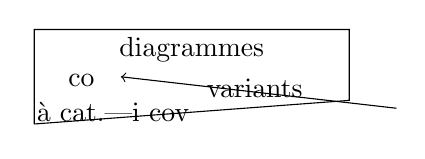
\begin{tikzpicture}
\draw (0,0)--(0,1.2)--(4,1.2)--(4,.3)--(0,0);
\node at (2,.95) {diagrammes};
\node at (.6,.55) {\unsure{co}};
\node at (2.8,.45) {\deleted{\unsure{variants}}};
\draw[->] (4.6,.2)--(1.1,.6);
\node at (1,.15) {\unsure{à cat.|i cov}};
\end{tikzpicture}}
% Inscription pâle renversée à 180 degrés au bord inférieur, barrée.
\deleted{\unsure{Théorie|Flèches}\ \illegible{1}\ \unsure{flèches|fibres}\quad II}
\scanpage{23}
% Folio d'archive : 22. Texte imprimé visible en transparence : verso, scan 024.
d) On veut que pour deux sous-catégories pleines $A',A''$ de $A$
\unsure{de réunion $A$}, qui sont soit des cribles soit des cocribles,
de réunion $A$, d'intersection $A_0$, l'application
\deleted{$\operatorname{Hom}($}
\[
\mathcal H(A)\longrightarrow\mathcal H(A')\times_{\mathcal H(A_0)}\mathcal H(A'')
\]
soit loc. \uline{surjective} sur les flèches
(elle a des chances d'être bijective sur les objets\ldots) i.e. pour
$\unsure{\xi|\zeta},\eta\in\operatorname{Ob}\mathcal H(A)$, on veut
\[
\operatorname{Hom}(\unsure{\xi|\zeta},\eta)\longrightarrow
\operatorname{Hom}(\unsure{\xi|\zeta}',\eta')
\times_{\operatorname{Hom}(\unsure{\xi|\zeta}_0,\eta_0)}
\operatorname{Hom}(\unsure{\xi|\zeta}'',\eta'')
\]
\uuline{surjectif}.
\margin{\figure{\begin{tikzpicture}\node[draw,ellipse] {Hot 7};\end{tikzpicture}}}
\margin{\uline{NB} Car on a déjà
$A=A'\amalg_{A_0}A''$ dans $(\mathrm{Cat})$}

On l'utilisera dans le cas de
\figure{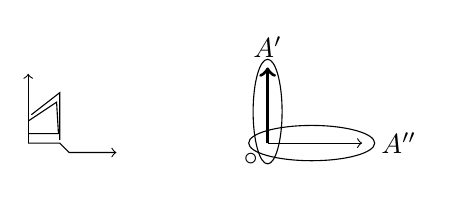
\begin{tikzpicture}[scale=.8]
\draw[->] (0,0)--(0,1.1);
\draw[->] (0,0)--(.5,0)--(.65,-.15)--(1.4,-.15);
\draw (0,.35)--(.45,.65)--(.48,.15)--(0,.15);
\draw (.05,.45)--(.5,.8)--(.5,.05);
\begin{scope}[xshift=3.8cm]
\node[below left] at (0,0) {$\circ$};
\draw[->,very thick] (0,0)--(0,1.2);
\draw[->] (0,0)--(1.5,0);
\node[above] at (0,1.2) {$A'$};
\node[right] at (1.65,0) {$A''$};
\draw (0,.5) ellipse (.23 and .83);
\draw (.7,0) ellipse (1 and .28);
\end{scope}
\end{tikzpicture}}
et le cas dual, et les produits par \unsure{tt élément|tout élément} $B$ de Cat
\scanpage{24}
% Folio d'archive : 23. Feuille dactylographiée réemployée.
\begin{tabular}{c@{\qquad\qquad}l}
UNIVERSITE DES SCIENCES ET TECHNIQUES & 15 avril 1983\\
DU LANGUEDOC &\\
U. E. R.\quad 5 &
\end{tabular}

\begin{center}
D.E.A.\quad DE\quad MATHEMATIQUES
\end{center}
\figure{\begin{tikzpicture}\draw[dashed] (0,0)--(5,0);\end{tikzpicture}}

Une réunion de tous les enseignants concernés aura lieu le
Jeudi 28 avril à 14 h 30 en salle 431 en vue d'adopter l'\uline{affiche des cours}
définitive pour 1983-1984.
% Le soulignement de « affiche des cours » est constitué de tirets.

Les professeurs responsables d'option sont priés d'apporter
à la réunion un programme écrit (10 lignes environ) et un horaire précis
(quantités d'heures annuelles, enseignants) pour chaque option.

\begin{flushright}P. MOLINO\end{flushright}
\scanpage{25}
% Folio d'archive : 24. Feuille entièrement diagrammatique.
% Petit diagramme, angle supérieur gauche.
\diagram{\begin{tikzcd}[column sep=small,row sep=small]
 & e\arrow[d] &\Omega Z\arrow[l]\arrow[d]\\
e\arrow[d] &\Omega Y\arrow[l]\arrow[d] &\Omega X\arrow[l]\arrow[d]\\
X\arrow[d] & Z\arrow[l]\arrow[d] &e\arrow[l]\\
Y &e\arrow[l] &
\end{tikzcd}}
% Grand escalier central ; tous les e, exposants et flèches conservés.
\diagram{\begin{tikzcd}[column sep=small,row sep=small]
&&&&e\arrow[d]&\Omega^3 Z\arrow[l]\arrow[d,"\Omega^3 g"]&\Omega^4 Y\arrow[l,"\Omega^3 h"']\arrow[d]\\
&&&e\arrow[d]&\Omega^3 Y\arrow[l]\arrow[d,"\Omega^2 h"']&\Omega^3 X\arrow[l,"\Omega^3 f"']\arrow[d]&e\arrow[l]\\
&&e\arrow[d]&\Omega^2 X\arrow[l]\arrow[d,"\Omega^2 f"']&\Omega^2 Z\arrow[l,"\Omega^2 g"']\arrow[d]&e\arrow[l]&\\
&e\arrow[d]&\Omega Z\arrow[l]\arrow[d,"\Omega g"']&\Omega^2 Y\arrow[l,"\Omega h"']\arrow[d]&e\arrow[l]&&\\
e\arrow[d]&\Omega Y\arrow[l]\arrow[d,"h"']&\Omega X\arrow[l,"\Omega f"']\arrow[d]&e\arrow[l]&&&\\
X\arrow[d,"f"']&Z\arrow[l,"g"']\arrow[d]&e\arrow[l]&&&&\\
Y&e\arrow[l]&&&&&
\end{tikzcd}}
% Petit angle isolé à droite.
\diagram{\begin{tikzcd}[column sep=small,row sep=small]
&\unsure{P|P'}\arrow[d]\\
p&Q\arrow[l]
\end{tikzcd}}
% Suite commencée immédiatement au-dessous du pli horizontal.
\diagram{\begin{tikzcd}[column sep=small]
Y&X\arrow[l]&Z\arrow[l]&\Omega Y\arrow[l]&{}\arrow[l]
\end{tikzcd}}
% Esquisse en perspective, moitié inférieure gauche : flèches, cercles
% et reprises de traits sont restitués comme dessin et non interprétés.
\figure{\begin{tikzpicture}[scale=.78]
\node[draw,circle,inner sep=1pt] (a) at (2,4.4) {$e$};
\node[draw,circle,inner sep=1pt] (b) at (1,3.5) {$e$};
\node[draw,circle,inner sep=1pt] (c) at (0,2.5) {$e$};
\node[draw,circle,inner sep=2pt] (x) at (0,1.5) {$\bullet$};
\node[left] at (x.west) {$X$};
\node[draw,circle,inner sep=2pt] (y) at (0,.4) {$\bullet$};
\node[left] at (y.west) {$Y$};
\node[draw,circle,inner sep=1pt] (d) at (1,.4) {$e$};
\node[draw,ellipse,inner sep=3pt] (e) at (2.15,1.5) {$e$};
\node[draw,ellipse,inner sep=3pt] (f) at (3,2.5) {$e$};
\coordinate (g) at (1,1.5);\coordinate (h) at (1,2.5);
\coordinate (i) at (2,2.5);\coordinate (j) at (2,3.5);
\coordinate (k) at (3,3.5);
\draw[->] (a)--(b);\draw[->] (b)--(c);\draw[->] (b)--(h);
\draw[->,thick] (h)--(c);\draw[->] (c)--(x);\draw[->] (x)--(y);
\draw[->] (d)--(y);\draw[->] (g)--(d);\draw[->] (h)--(g);
\draw[->,thick] (g)--(x);\draw[->] (e)--(g);\draw[->] (e)--(d);
\draw[->] (i)--(e);\draw[->] (f)--(e);\draw[->,thick] (f)--(i);
\draw[->] (i)--(h);\draw[->] (j)--(i);\draw[->,thick] (j)--(b);
\draw[->] (k)--(j);\draw[->] (k)--(f);\draw[->] (a)--(j);
\draw[->] (j)--(g);\draw[->] (2.8,3.8)--(2.8,5.2);
\draw[->] (3.6,4.4)--(3.6,3.7);
\draw[very thick,rounded corners=3pt] (1.9,3.5)--(1.9,4.6)--(2.1,4.6)--(2.1,3.7)--(3,3.7)--(3.3,2.6)--(3.3,1.1);
\draw (1.75,3.6)--(1.8,4.8);\draw (3.1,3.6)--(3.1,.6);
\draw (.4,4.7)--(1.9,4.7);\draw (.4,4.05)--(2.8,4.05);
\draw[dashed] (2.9,4.3)--(3.5,4.3);\draw[dashed] (3.2,3.5)--(3.6,3.5);
\end{tikzpicture}}
% Deux points isolés, à droite sous la suite commencée.
\diagram{\begin{tikzcd}[column sep=small]\bullet&\bullet\end{tikzcd}}
% Deux petits carrés déformés, à droite de l'esquisse.
\diagram{\begin{tikzcd}[column sep=small,row sep=small]
e\arrow[d,thick]&{}\arrow[dd,dashed]&\bullet\arrow[ll,dashed]\\
X\arrow[d]&&e\arrow[ll,thick]\arrow[dl]\arrow[u,dotted,very thick]\\
Y&e\arrow[l]&
\end{tikzcd}}
% Longue suite inférieure avec les e intercalés ; la suite se poursuit hors dessin.
\diagram{\begin{tikzcd}[column sep=.8em,row sep=1.2em]
&&e\arrow[dl]&&e\arrow[dl]&&e\arrow[dl]&&e\arrow[dl]&&\\
Y&X\arrow[l]&Z\arrow[l]\arrow[dl]&\Omega Y\arrow[l]\arrow[ul]&\Omega X\arrow[l]\arrow[dl]&\Omega Z\arrow[l]\arrow[ul]&\Omega^2 Y\arrow[l]\arrow[dl]&\Omega^2 X\arrow[l]\arrow[ul]&\Omega^2 Z\arrow[l]\arrow[dl]&\Omega^3 Y\arrow[l]\arrow[ul]&{}\arrow[l]\\
&e\arrow[ul]&&e\arrow[ul]&&e\arrow[ul]&&e\arrow[ul]&&&
\end{tikzcd}}
% Reprise rayée sous l'extrémité gauche de la suite.
\deleted{\figure{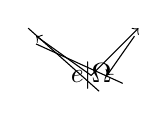
\begin{tikzpicture}
\node at (0,0) {$\unsure{e|\Omega}$};
\draw[->] (0,0)--(-.7,.5);\draw[->] (0,0)--(.6,.6);
\draw (-.7,.4)--(.4,-.1);\draw (-.8,.6)--(.1,-.2);
\draw[->] (.55,.5)--(.2,0);
\end{tikzpicture}}}
\scanpage{26}
% Folio d'archive : 25. Circulaire imprimée et dactylographiée, tampons et signature.
REPUBLIQUE FRANÇAISE

Ministère de la recherche et de l'industrie
\figure{\begin{tikzpicture}\draw (0,0)--(12,0);\end{tikzpicture}}
Mission scientifique et technique\hfill Paris, le\quad 30 Mars 1983
\figure{\begin{tikzpicture}\draw (0,0)--(12,0);\end{tikzpicture}}

1 rue Descartes\\
75231 Paris Cedex 05\\
Tél. 634'33 33 / 634 35 35\\
Telex MRIACR 204 643 F

Réf.

% Tampon de réception, à droite du bloc d'adresse.
\figure{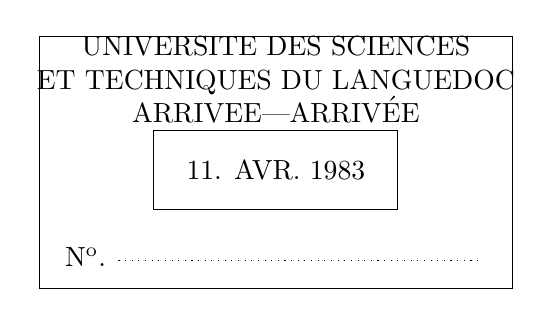
\begin{tikzpicture}
\draw (0,0) rectangle (6,3.2);
\node[align=center] at (3,2.65) {UNIVERSITE DES SCIENCES\\ET TECHNIQUES DU LANGUEDOC\\\unsure{ARRIVEE|ARRIVÉE}};
\draw (1.45,1) rectangle (4.55,2);
\node at (3,1.5) {11. AVR. 1983};
\node[anchor=west] at (.2,.4) {N\textsuperscript{o}.};
\draw[dotted] (1,.35)--(5.6,.35);
\end{tikzpicture}}

Messieurs, Mesdames les Directeurs de Formation de Recherche,

Le développement des techniques au service de la recherche dans
le domaine des Sciences de la Vie nous amène à nous préoccuper de la
planification de l'équipement en matériels semi-lourds de nos laboratoires
(nous entendons par matériels semi-lourds des appareils dont le prix
d'achat est compris entre 0,5 et 5 millions de francs).

Nous désirons tout d'abord faire une mise au point sur l'état actuel
du parc des appareils semi-lourds et de leur ancienneté, deuxièmement
connaitre les besoins actuels et futurs pour ces types d'appareils, dont
la liste non exhaustive est ci-jointe.

Pour chaque type d'appareils existant dans votre laboratoire,
veuillez nous préciser la date d'achat et la source du financement de cet
appareil et d'autre part veuillez nous faire savoir quels sont vos
besoins actuels et vos besoins prévisibles pour les prochaines années
(84-89) concernant ces équipements semi-lourds.

Une fiche réponse est jointe à cette lettre, elle devrait nous être
retournée si possible par retour du courrier.

L'ensemble des réponses seront dépouillées avant la fin avril 1983
et vous serez personnellement informé des résultats de l'enquête et des
prospectives.

Je vous remercie d'avance pour votre diligente collaboration, et
vous prie de croire, Cher Collègue, à mes sentiments les meilleurs.

% Signature manuscrite, puis nom dactylographié.
\figure{
\begin{tikzpicture}
\node[font=\itshape] at (2,.6) {D. Pantaloni};
\draw (0,.2)..controls (1,.1) and (.8,.9)..(.3,1)..controls (.25,.6) and (.45,.2)..(.45,.35);
\draw (1.3,.35)..controls (1.1,1.3) and (2,1.45)..(1.8,1.1)..controls (1.7,1) and (1.3,1)..(1.4,.2);
\end{tikzpicture}}
\begin{flushright}D. Pantaloni\end{flushright}

% Mention de transmission encadrée, en bas à gauche.
\figure{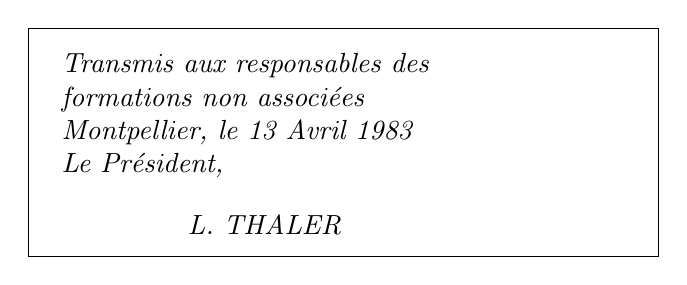
\begin{tikzpicture}
\draw (0,0) rectangle (8,2.9);
\node[anchor=north west,align=left,font=\itshape] at (.3,2.7)
{Transmis aux responsables des\\formations non associées\\Montpellier, le 13 Avril 1983\\Le Président,};
\node[font=\itshape] at (3,.4) {L. THALER};
\end{tikzpicture}}
% Tampon circulaire chevauchant le cadre et la première ligne du P.S.
\figure{
\begin{tikzpicture}
\draw (0,0) circle (1.7);\draw (0,0) circle (1.25);
\node[align=center] at (0,.95) {ACADEMIE DE MONTPELLIER};
\node[align=center,font=\small] at (0,-.15)
{UNIVERSITE\\DES SCIENCES ET\\TECHNIQUES DU\\LANGUEDOC};
\fill (0,-1.45) circle (2pt);
\end{tikzpicture}}

P.S. Une seconde feuille réponse est jointe à cette lettre afin que
vous puissiez la diffuser éventuellement auprès de collègues
universitaires qui n'appartiendraient pas à une formation de recherche
du C.N.R.S. où de l'I.N.S.E.R.M.
